\subsection{Approximations and Round Off Errors - Chapter 3}

\begin{enumerate}
  
  \item {\bf Significant Figures}
  
   Significant Figures or Digits is the number or amount of
   information we have to convey a number. For example, take a look at
   your phone or your watch. What time is it? My watch says 13:11
   PM. That is it is the 13th hour of the day, the 11th minute of the
   hour. How many seconds on the minute is it? I don't know. My watch
   doesn't tell me. Next time you get into your car look at how many
   miles your car has. Mine says 67,611.1, that is pretty accurate but
   what if I converted that number to feet? 5280 feet = 1 mile so
   67,611.1 = 356,986,608 feet. Where did the decimal place go?
   Certainly I haven't traveled exactly the many feet. The reason is
   because I don't have enough significant digits. What about pi? How
   many decimal places can you list? How many does your calculator
   list? The fact is we all make approximation and computers are no
   different. They hold a certain number of digits in its memory to 
   represent a number. The goal is that the number has enough numbers
   to be accurate as well as precise.

   \item {\bf Accuracy and Precision}

     {\it Accuracy}: how closely a computed or measured value agrees
     with the true value
     {\it Precision}: how closely multiple measurements agree with
     each other

     Let's go back to the watch again. How accurate is your watch? My
     watch says 1:17PM, according to Google it is 1:18:22 PM. So my
     watch was off by 1 minute and 22 seconds. My phone says 1:18PM so
     my phone is only off by 22 seconds. Thus, my phone is more
     accurate then my watch but this is because my phone is
     automatically synchronized with the world clock. However, both my
     watch and my phone are arguably just as precise.

  \item {\bf Error Definitions} 

    Let's assume for the moment that I am 6'0" tall. I go to the
    doctor and the doctor tells me I am 72.25". Using the equation
    below we can determine the absolute error in my doctor's measurement.

    \begin{equation}
      absolute\_error = |actual - computed|
    \end{equation}

    6 feet is 72 inches thus the absolute error is 0.25". Sometimes
    however it is not enough to compute the absolute error. For
    example, assume you are measuring a 1000 foot building. Does it
    really matter that you are off by a quarter of an inch? It might
    matter given the circumstances but it matters a lot more when you
    are measuring a 2 foot long beam to put in your house. Thus, the
    percent error is defined as such to account for the difference in
    scale.
    
    \begin{equation}
      percent\_error = 100*absolute\_error/actual
    \end{equation}

    Thus the percent error in my height is 0.347\%. Notice, that I only
    saved four significant digits since my measurement was only
    accurate to 4 significant digits. 

  \item {\bf Computer Representation of Numbers}
  
    Computers although powerful have the same fundamental problem as
    above. Let's assume for the sake of this argument that you have a
    book in your hand and a pencil. You are only allowed to write two
    numbers on each page. Some one asks you what 5 times 5 is. You
    open up page 1 and write the number 5 on page 1. Then you turn to
    page two and write the number 5 on page 2. You then compute 5
    times 5 in your head and arrive at the number 25 and write 25 on
    page three. The same person then says what is 25 times 5. You
    again compute in your head that 5 times 25 is 125. You turn to
    page 4, you pause and scratch your head, you can only write down
    two numbers, what should you do? Your most logical result is to
    throw out the 1 and write down 25. You then say that 25 times 5 is
    25. This is how a computer works. The person asking you questions
    is a mouse and/or keyboard. The signals from the mouse and
    keyboard are sent through the motherboard to the Central
    Processing Unit (CPU) much like your brain. The motherboard is
    like your entire body connecting everything together. Think of it
    as your central nervous system. When you computed 5 times 5 you
    did that in your head but note that your brain has long term and
    short term memory. The short term memory is like the computers RAM
    or Random Access Memory. The long term memory is like the Hard
    disk drive or Harddrive (HDD). The pages in your book are
    different locations or hexadecimal addresses the computers
    harddrive. So then how does the computer actually compute? Well
    let's start with how we represent numbers in base 10. If I write
    5 in base 10 I would have

    \begin{equation}
      0 \times (10^1) + 5 \times (10^0)
    \end{equation}

    the number 25 would then be

    \begin{equation}
      2 \times (10^1) + 5 \times (10^0)
    \end{equation}

    You can now see why the number 125 is impossible to represent if I
    can only hold two digits. If I could hold 3 digits I could
    represent 125 using this equation

    \begin{equation}
      1 \times (10^2) + 2 \times (10^1) + 5 \times (10^0)
    \end{equation}

    Fractions are simple too. Say we return to my height of 72.25". In
    base 10 that would be 

    \begin{equation}
      7 \times (10^1) + 2 \times (10^0) + 2 \times (10^{-1}) + 5
      \times (10^{-2}) = 72.25
    \end{equation}

    We however have adopted base 10 so easily that we just leave off
    the $10^x$ and just report the numbers. Wouldn't it be great if we
    could just get computers to do this? It would only have to
    represent the number 0-9 and then it would be able to represent
    any number in the number line provided it could store that many
    significant digits. The problem with this is in the
    circuitry. Computers are either on (1) or off (0). This means they
    can't represent the number 0-9 they can only represent the numbers
    0 and 1. Most computers operate on +5V for on and -5V for
    off. Thus if the computer receives +5V it is a 1 and -5V for an
    off. So if 0-9 (10 numbers) is base 10, what is 0-1 (2 numbers)?
    That's base 2 which is called binary. The conversion from binary
    to base 10 is difficult so let's just start with a few
    examples. Say I want to convert $101_2$ to base 10. The subscript
    2 indicates base 2. Well that would be

    \begin{equation}
      1 \times (2^2) + 0 \times (2^1) + 1 \times (2^0) = 5
    \end{equation}

    This number above is 3 bits of data. 8 bits equals 1 byte. 8
    bytes is equal to 64 bits. So if you have a 64 bit machine it
    means that the computer is capable of reading 64 bits of data. My
    computer represents all number uses 8 bytes or 64 bits. MATLAB on
    the other hand using floating point precision. So, the 0-51st bit
    is used for fractions, $2^{-1}$ all the way to $2^{-51}$, the 52st bit to
    the 62nd bit is used for the exponent except it is biased by
    1023 thus the maximum number that MATLAB can predict is
    $2^{1024}$. Finally, the 63rd bit is the sign of the number. 

    \begin{figure}[htb]
      \begin{center}
        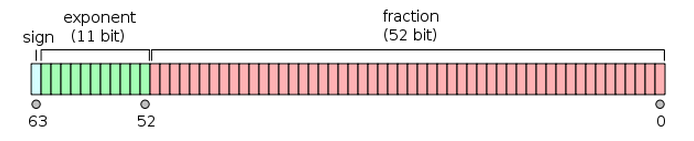
\includegraphics[height=0.2\textwidth,width=0.9\textwidth]{Graphics/Floating_Point_Precision}
      \end{center}
    \end{figure}

    Thus a number would be represented using the formula below.

    \begin{equation}
      (-1)^{(bit_{63})}(1+\sum\limits_{i=1}^{52}bit_{52-i}2^{-i})\times 2
      ^{e-1023}
    \end{equation}
    
    where e is determined by bits 52-63. The maximum number can be
    computed by noting that the exponent has 11 bits. The maximum
    exponent number represented by 11 bits is $2^{11}-1=2047$. The biased
    exponent is then $2047-1023=1024$. Note that if you type
    $2^{1024}$ in MATLAB you will get Inf. However if you type
    $2^{1023}*1.99999$ you will get the value of {\it realmax}. The largest number is
    still $2^{1024}$. The smallest number is actually
    $2^{-1022}$. This is represented with a 1 in the exponent field
    such that e=1 and e-1023 = -1022. It is actually possible to get
    smaller numbers on a computer by using denormalized numbers. That
    is when using denormalized number the exponent is assumed to be
    zero. Thus e=0 and the number can be as small as
    $2^{-1023}$. However, with this representation it is possible to
    truncate the equation above to the following denormalized version

    \begin{equation}
      (-1)^{(bit_{63})}(\sum\limits_{i=1}^{52}bit_{52-i}2^{-i})\times 2
      ^{-1023}
    \end{equation}
    
    Thus the smallest number is actually $2^{-1023}*2^{-52}$. Again,
    MATLAB will return a zero if you type this number in but
    $2^{-1023}*2^{-51}*(1.999)^{-1}$ is pretty close. 

  \item {\bf Computer Representation of Characters}

    Numbers are all well and good but I also want to be able to write
    text. So if I write 'hello' how does my computer represent it?
    Well back in the 1960s when binary representation was first coming
    out they came up with the American Standard or Character
    Information Interchange (ASCII). If you take the upper/lower case
    alphabet (26*2), plus punctuation like $?$ or \# and some
    non-printing characters like {\it backspace} or {\it del} you find
    that you need something like 100 characters. In binary that means
    you need 7 bits which leads to $2^7-1=127$. In order to organize
    the characters properly the mathematicians decided to make the
    letter 'A' = 65. The reason why can be explained by computing the
    binary equivalent for A.

    \beq
    \begin{matrix}
    A = 65_{10} = 10~00001_2 \\
    B = 66_{10} = 10~00010_2 \\
    C = 67_{10} = 10~00011_2 \\
    \hdots \\
    etc,etc,etc
    \end{matrix}
    \eeq

    Similary, lower case 'A' is 'a' or 97. Again converting to binary
    leads to

    \beq
    \begin{matrix}
    a = 97_{10} = 11~00001_2 \\
    b = 98_{10} = 11~00010_2 \\
    c = 99_{10} = 11~00011_2 \\
    \hdots \\
    etc,etc,etc
    \end{matrix}
    \eeq

    Thus, it is really easy to compute the letters based on the binary
    number. If you'd like to put a string together you can just
    combine binary numbers. For example, let's convert 'cat' to
    binary.

    \beq
    \begin{matrix}
      c = 99_{10} = 11~00011_2 \\
      a = 97_{10} = 11~00001_2 \\
      t = 116_{10} = 11~10100_2 \\
    \end{matrix}
    \eeq

    What's really cool is that if you want to capitalize the word
    'cat' in binary you simply need to decrement the second bit to 0
    thus 'CAT' in binary is simply
    $10~00011_2,10~00001_2,10~110100_2$. In MATLAB/Octave it is really
    easy to check your work when performing these actions. To get the
    ASCII code simply type 

    \beq
    double('inert\_letter\_here')
    \eeq

    Try it out and see what you get for different letters. You can
    also do strings like your name for example.

    \beq
    double('carlos') =
    99_{10},97_{10},114_{10},108_{10},111_{10},115_{10}
    \eeq

    Even cooler you can convert from decimal to binary using the {\it
      dec2bin} function thus you can type

    \beq
    dec2bin(double('carlos')) = \begin{matrix} 11~00011_2
      \\ 11~00001_2 \\ 11~10010_2 \\ 11~01100_2
      \\ 11~01111_2 \\ 11~10011_2 \end{matrix}
    \eeq
    
    Note, you can also convert to characters by typing in a number
    from 0 to 127 using the {\it char} function. For example if I type
    {\it char(33)} I get the exclamation point. Try a few and see what
    you get.

    \beq
    char(33) =~!
    \eeq

    So for a long time this was all well and good but then people
    wanted to be able to represent other characters like latin, greek,
    roman for computation. Well 127 characters wasn't enough but 8 bit
    computers came out and then we had 255 characters. At the time
    this was enough for every language. The problem is that the
    Norwegians adopted a different standard rather than ASCII, the
    Japanese came up with their own multibyte data structure. This was
    fine back in the 70s because typically back then you would just
    print your document and fax it or mail it. Imagine if you write
    something in ASCII and send the binary file to someone using a
    different format. It's like speaking a different language they
    wouldn't understand. Well this didn't matter until the late 70s
    early 80s when the World Wide Web opened up and then suddenly
    people are reading languages in different binary format. 

    \item {\bf Unicode Format - UTF}

      So what did people do? They adopted the Unicode format which is
      a variable length format. Currently UTF-8 is the most standard
      (circa 2015) which uses 1-4 8 bits strings = 8-32 bits = 1-4
      bytes per number. Using this variable length format you can
      represent all characters you can imagine. All 1,112,064
      characters in all the human languages. However, MATLAB/Octave
      said they do not need 32 bits of information so Octave decided
      to use 8 bits (255 characters) and MATLAB decided to use 16 bits
      (65,535 characters). In MATLAB you can test this by typing {\it
        uint16} for example

      \beq
      x = uint16('g') = 103_{10} = 2~bytes
      \eeq
      
      yields the number 103 using 16 bits or 2 bytes. You can also
      similarly use the 8 bit standard using the function {\it uint8} 

      \beq
      x = uint8('g') = 103_{10} = 1~byte
      \eeq
      
      The standard character format in MATLAB is the character which
      uses 2 bytes. Octave's standard for characters is 1 byte. This
      is just what happens when you have multiple people writing
      different code. MATLAB as it is however allows you to use multiple
      different formats should you so desire. Some examples include
      'UTF-7','UTF-8','UTF-16' or 'ISO-8859-1' to name a few.

\end{enumerate}

